
\chapter{Computing basics}

\textbf{What is a computer?}

A computer is a machine that can be programmed to automatically carry
out sequences of arithmetic or logical operations (computation). Modern digital
electronic computers can perform generic sets of operations known
as programs. These programs enable computers to perform a wide range of
tasks. The term computer system may refer to a nominally complete computer
that includes the hardware, operating system, software,
and peripheral equipment needed and used for full operation;

A Computer cluster is a group of computers that are linked and function
together.

\begin{minipage}[t]{0.45\textwidth}
    \begin{figure}[H]
        \centering
        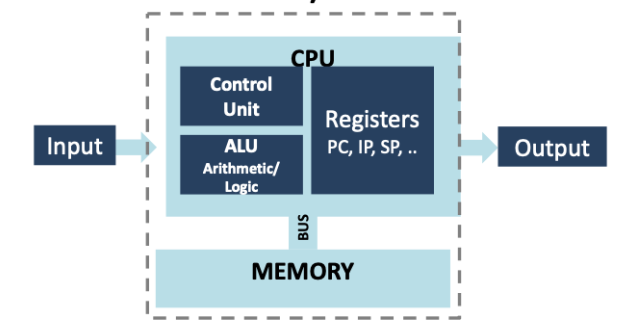
\includegraphics[width=0.9\textwidth]{assets/fig16.png}
        \caption{Serial Computer}
    \end{figure}
\end{minipage}
\begin{minipage}[t]{0.45\textwidth}
    \vspace{0.5cm}
    A \textbf{serial computer} is a computer that processes data one bit at a time. This is in contrast to a parallel computer, which processes multiple bits at the same time. Serial computers are much slower than parallel computers, but they are also much simpler and cheaper to build.
\end{minipage}

Today, the most common form of computer is a digital computer, and computing
machines have been an integral part of the business and engineering
world since the late 20th century. Computers are used in a wide range of
applications, including data processing, business management, and word
processing. They are also used in scientific research, engineering, and
medicine. Computers are used to control industrial processes and to
simulate complex systems. Modern computers are capable of performing
a wide range of tasks, from simple arithmetic to complex calculations.

\begin{minipage}[t]{0.45\textwidth}
    \vspace{1cm}
    A \textbf{parallel computer} is a computer that processes data multiple bits at the same time. This is in contrast to a serial computer, which processes data one bit at a time. Parallel computers are much faster than serial computers, but they are also much more complex and expensive to build.
\end{minipage}
\begin{minipage}[t]{0.45\textwidth}
    \begin{figure}[H]
        \centering
        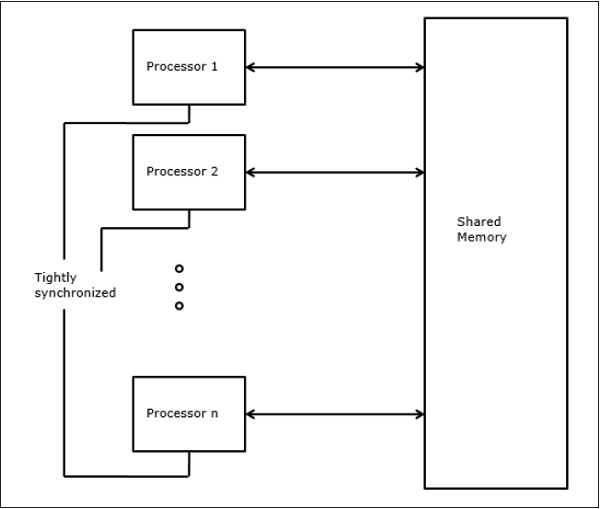
\includegraphics[width=0.9\textwidth]{assets/fig17.jpg}
        \caption{Parallel Computer}
    \end{figure}
\end{minipage}

\newpage 
There are two main types of parallel computers: shared memory and distributed memory. In a shared memory system, all processors share the same memory. In a distributed memory system, each processor has its own memory. Parallel computers are used in a wide range of applications, including scientific research, engineering, and business.
\begin{itemize}
    \item \textbf{Shared memory:} In a shared memory system, all processors share the same memory. This allows processors to communicate with each other by reading and writing to the same memory locations. Shared memory systems are typically used in applications that require high performance and low latency, such as scientific research and engineering.
        \begin{itemize}
            \item Uniform Memory Access (UMA): each processor has uniform access to memory.
            \begin{figure}[H]
                \centering
                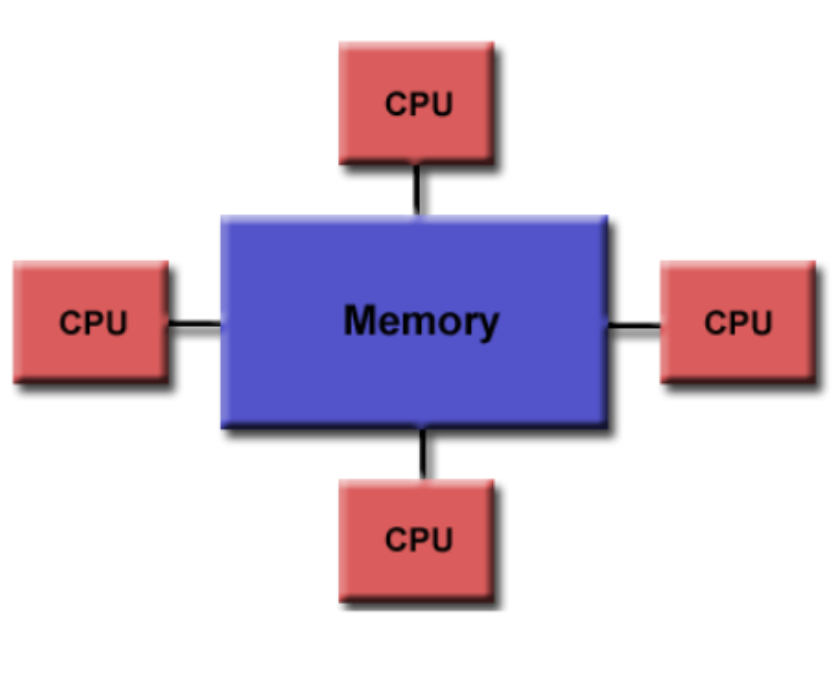
\includegraphics[width=0.4\textwidth]{assets/fig18.png}
                \caption{Uniform Memory Access (UMA)}
            \end{figure}
            \item Non-Uniform Memory Access (NUMA): time for memory access depends on location of data. Local access is faster than non-local access. 
            \begin{figure}[H]
                \centering
                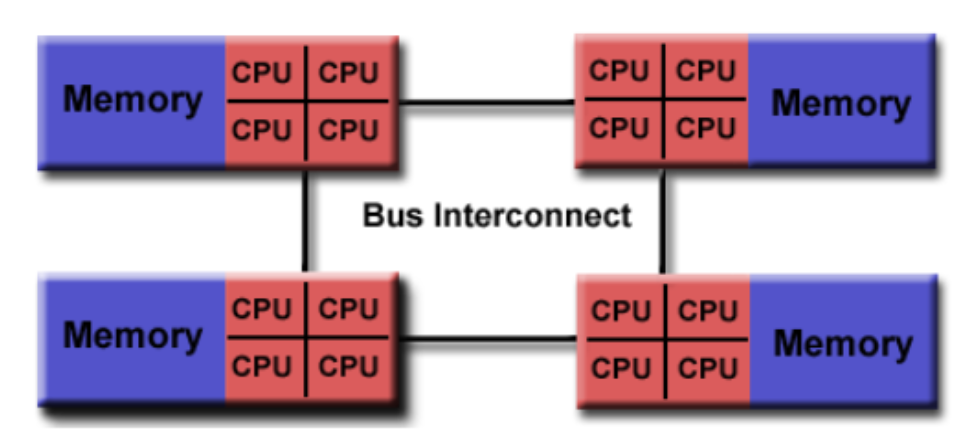
\includegraphics[width=0.4\textwidth]{assets/fig19.png}
                \caption{Non-Uniform Memory Access (NUMA)}
            \end{figure}
        \end{itemize}
    \item \textbf{Distributed memory:} In a distributed memory system, each processor has its own memory. This allows processors to communicate with each other by sending messages over a network. Distributed memory systems are typically used in applications that require scalability and fault tolerance, such as large-scale data processing and cloud computing.
    \begin{figure}[H]
        \centering
        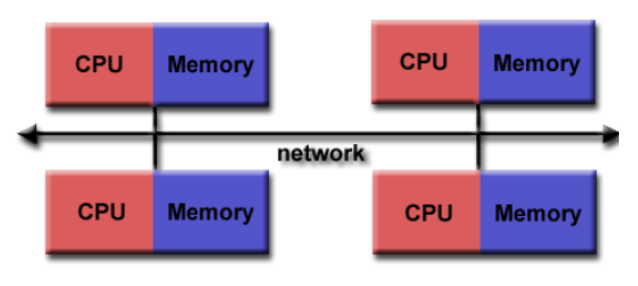
\includegraphics[width=0.4\textwidth]{assets/fig20.png}
        \caption{Distributed Memory}
    \end{figure}
\end{itemize}

\section{Cluster}

A computer cluster is a group of computers that are linked and function
together. The components of a cluster are usually connected to each other
through fast local area networks, with each node running its own instance
of an operating system. Clusters are used for a wide range of applications,
including scientific research, engineering, and business. They are
also used in cloud computing and high-performance computing.

\begin{figure}[H]
    \centering
    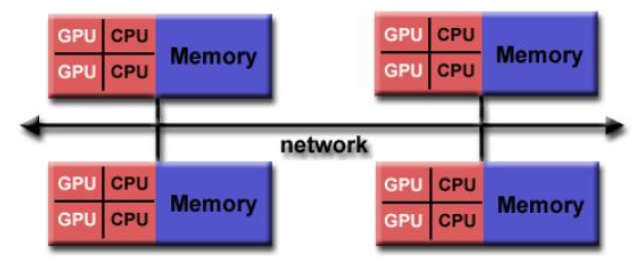
\includegraphics[width=0.6\textwidth]{assets/fig21.png}
    \caption{Computer Cluster}
\end{figure}

Compopnents of a cluster:
\begin{itemize}
    \item \textbf{Nodes:} A node is a single computer in a cluster. Each node has its own processor, memory, and storage. Nodes are connected to each other through a network.
    \item \textbf{Network:} The network is the communication infrastructure that connects the nodes in a cluster. The network allows nodes to communicate with each other and share data.
    \item \textbf{Operating System:} Each node in a cluster runs its own instance of an operating system. The operating system manages the resources of the node and provides an interface for running applications.
    \item \textbf{Applications:} Applications are programs that run on the nodes in a cluster. Applications can be parallelized to take advantage of the resources of the cluster.
\end{itemize}

\begin{figure}[H]
    \centering
    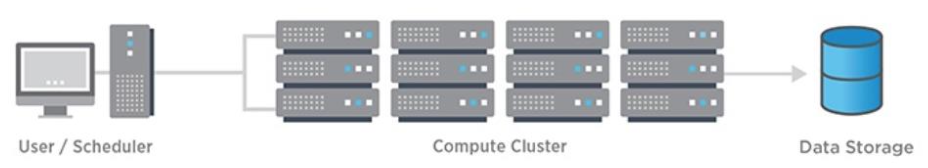
\includegraphics[width=0.6\textwidth]{assets/fig22.png}
    \caption{Components of a Cluster}
\end{figure}

\begin{minipage}[t]{0.45\textwidth}
    \vspace{2.5cm}
    What does a node contain?
\end{minipage}
\begin{minipage}[t]{0.45\textwidth}
    \begin{figure}[H]
        \centering
        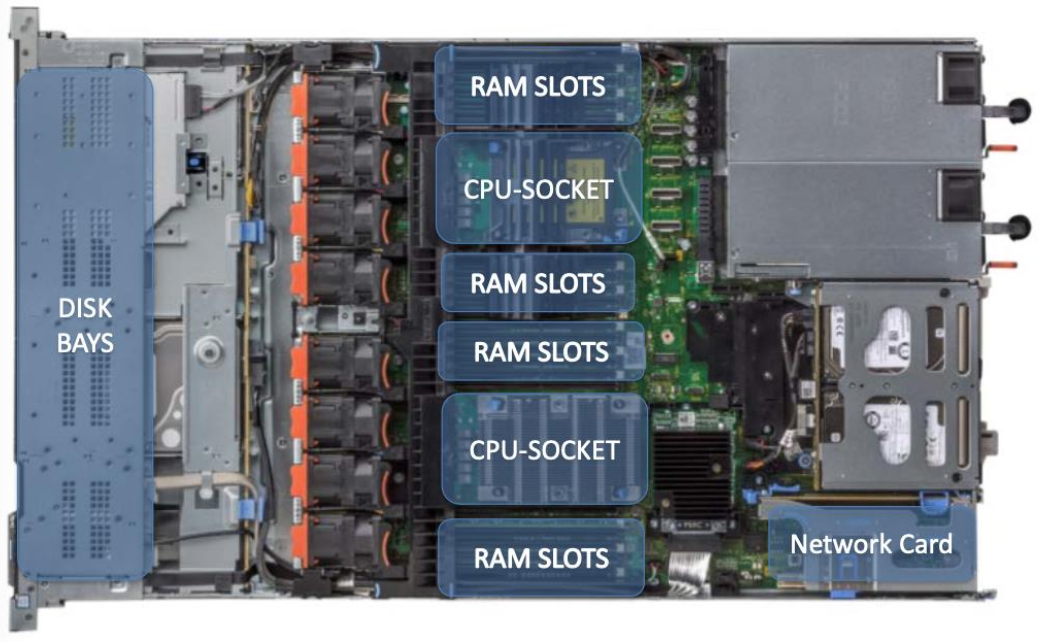
\includegraphics[width=0.9\textwidth]{assets/fig23.png}
        \caption{Node Components}
    \end{figure}
\end{minipage}

\begin{minipage}[t]{0.45\textwidth}
        \begin{figure}[H]
            \centering 
            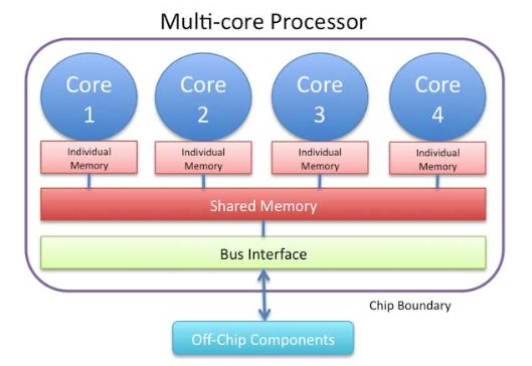
\includegraphics[width=0.9\textwidth]{assets/fig24.png}
            \caption{multicore CPU}
        \end{figure}
\end{minipage}
\begin{minipage}[t]{0.45\textwidth}
\vspace{1cm}
\textbf{CPU are multicore proccessors.} Because of power, heat dissipation, ..., increasing tendency to actually lower clock frequency but pack more computing cores onto a chip. These cores will share some resources, i.e. memory, network, disk, etc. but are still capable of independent calculations. 
\end{minipage}

\begin{definitionblock}[Core]
    A core is the smallest unit of computing, having one or more (hardware/software) threads and is responsible for executing instructions.
\end{definitionblock}

\textbf{Intel \textregistered Hyper-Threading Technology} uses processor resources more efficiently, enabling multiple threads to run on each core. The OS "sees two cores and transparently try to execute two programs on two different "cores". 

A bit of jargon:
\begin{itemize}
    \item \textbf{Multiprocessor} = server with one or more than 1 CPU 
    \item \textbf{Multicore} = CPU with more than 1 core
    \item \textbf{Processor} = CPU = socket = chip
\end{itemize}

\begin{minipage}[t]{0.35\textwidth}
    \begin{figure}[H]
        \centering
        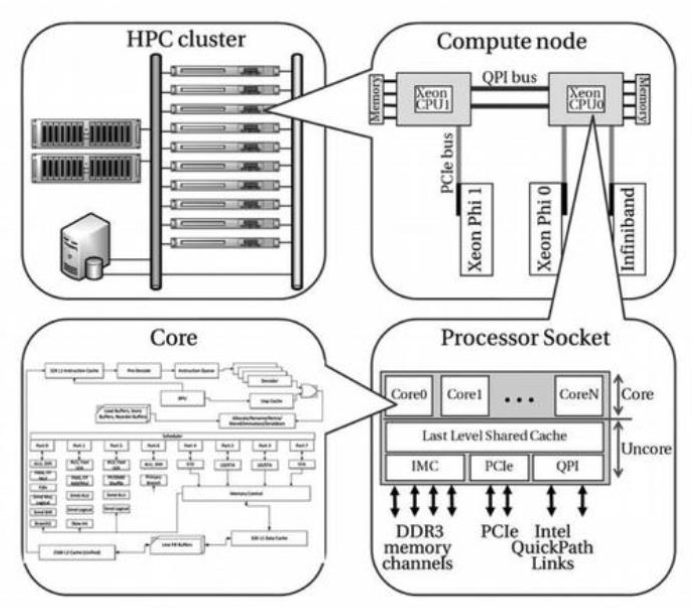
\includegraphics[width=0.9\textwidth]{assets/fig25.png}
        \caption{Computing Cluster}
    \end{figure}
\end{minipage}
\begin{minipage}[t]{0.55\textwidth}
    \begin{figure}[H]
        \centering
        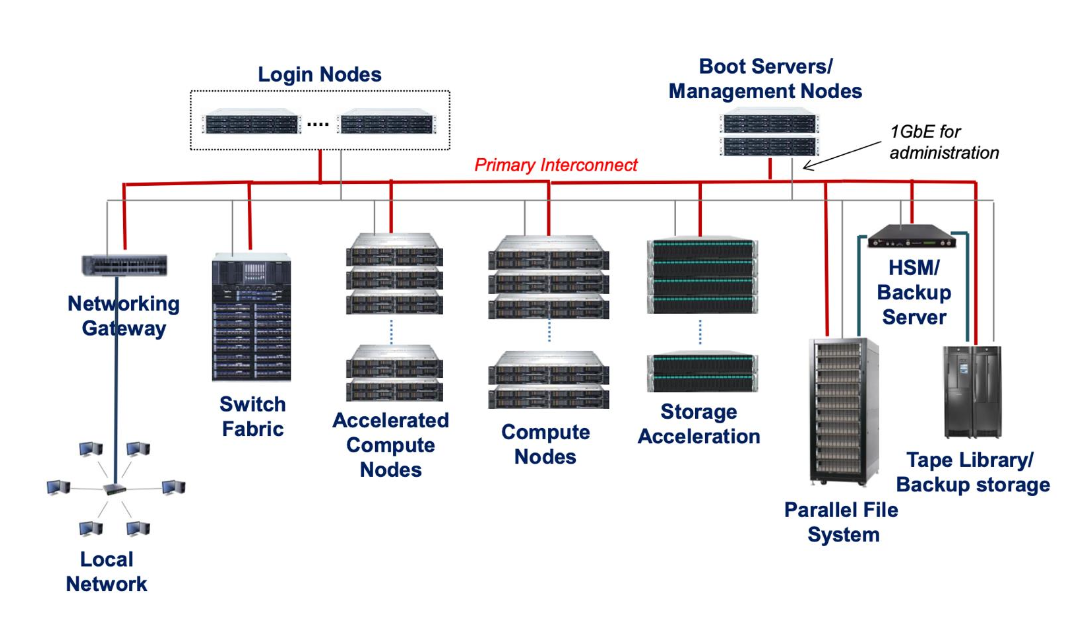
\includegraphics[width=0.9\textwidth]{assets/fig26.png}
        \caption{HPC cluster}
    \end{figure}
\end{minipage}


The \textbf{scheduler} is a software component that manages the resources of a
cluster. It is responsible for allocating resources to applications and
ensuring that they run efficiently. The scheduler is typically part of the
operating system of the cluster and is responsible for managing the
resources of the cluster, such as CPU, memory, and storage. The scheduler
uses algorithms to allocate resources to applications based on their
requirements and priorities.

\begin{itemize}
    \item It allocates exclusive or non-exclusive access to the resouces (the nodes) to users during a limited amout of time so that they can perform their work
    \item It abitrates contention for resources by managina a queue of pending work 
    \item It permits to schedule jobs for users on the cluster resources 
\end{itemize}

A user job is characterized by:
\begin{itemize}
    \item the number of nodes 
    \item the number of CPU cores 
    \item the memory requested 
    \item the walltime 
    \item the launcher script, which will initiate your task 
\end{itemize}

A \textbf{partition} is a group of compute nodes, with specific usage characteristics, like time limits and maximum number of nodes per job.

